% CVPR 2023 Paper Template
% based on the CVPR template provided by Ming-Ming Cheng (https://github.com/MCG-NKU/CVPR_Template)
% modified and extended by Stefan Roth (stefan.roth@NOSPAMtu-darmstadt.de)

\documentclass[10pt,twocolumn,letterpaper]{article}

%%%%%%%%% PAPER TYPE  - PLEASE UPDATE FOR FINAL VERSION
%\usepackage[review]{cvpr}      % To produce the REVIEW version
\usepackage{cvpr}              % To produce the CAMERA-READY version
%\usepackage[pagenumbers]{cvpr} % To force page numbers, e.g. for an arXiv version

% Include other packages here, before hyperref.
\usepackage{graphicx}
\usepackage{amsmath}
\usepackage{amssymb}
\usepackage{booktabs}
\usepackage{listings}
% It is strongly recommended to use hyperref, especially for the review version.
% hyperref with option pagebackref eases the reviewers' job.
% Please disable hyperref *only* if you encounter grave issues, e.g. with the
% file validation for the camera-ready version.
%
% If you comment hyperref and then uncomment it, you should delete
% ReviewTempalte.aux before re-running LaTeX.
% (Or just hit 'q' on the first LaTeX run, let it finish, and you
%  should be clear).
\usepackage[pagebackref,breaklinks,colorlinks]{hyperref}
\usepackage{indentfirst}
\usepackage{tabularx}
% Support for easy cross-referencing
\usepackage[capitalize]{cleveref}
\crefname{section}{Sec.}{Secs.}
\Crefname{section}{Section}{Sections}
\Crefname{table}{Table}{Tables}
\crefname{table}{Tab.}{Tabs.}
\lstset{
	basicstyle=\fontsize{8}{10}\selectfont\ttfamily
}
\graphicspath{{images}}
\def\wrt{w.r.t.\@\xspace}

%%%%%%%%% PAPER ID  - PLEASE UPDATE
\def\cvprPaperID{*****} % *** Enter the CVPR Paper ID here
\def\confName{CVPR}
\def\confYear{2023}


\begin{document}

%%%%%%%%% TITLE - PLEASE UPDATE
\title{Deep Learning Fundamentals\\
	Assignment 2 - Bird Classification: CNN and Beyond}

\author{Ziyang Ye\\
The University of Adelaide\\
{\tt\small a1707805@adelaide.edu.au}}
\maketitle

%%%%%%%%% ABSTRACT
\begin{abstract}
	This project mainly employs Convolutional Neural Networks (CNNs), a milestone of modern Computer Vision and Deep Learning, to revolutionize the identification of endemic bird species.
	CNN, with its automated feature extraction and hierarchical feature learning, enables the model to adeptly handle the complexities and variations inherent in avian imagery, ensuring nuanced and accurate species identification. 
	The integration of deep learning facilitates a seamless fusion of technological innovation with practical conservation efforts, leveraging platforms like eBird to enrich the model with a wealth of real-world observational data. 
	This project not only advances wildlife identification technology but also promotes a comprehensive exploration and monitoring of worldwide avian biodiversity, bolstering global conservation and education efforts.
\end{abstract}

%%%%%%%%% BODY TEXT
\section{Introduction}
\label{sec:intro}
The advent of deep learning, particularly Convolutional Neural Networks, has heralded a transformative era in the realm of image classification tasks, including the nuanced domain of bird species identification. This project embarks on a meticulous exploration of various CNN architectures, such as VGG and ResNet, alongside innovative architectures like Vision Transformers (ViT) and Swin Transformers. By intertwining these diverse architectures with an array of data augmentation strategies and training techniques, this study aims to unravel the comparative advantages and limitations of each approach in the context of bird classification.

Bird classification holds profound significance, serving as a linchpin in conservation efforts, scientific research, and educational outreach. Accurate and automated identification of bird species fosters enhanced monitoring and understanding of avian biodiversity, thereby bolstering conservation initiatives and facilitating informed decision-making in habitat preservation and species protection. In this light, the application of deep learning and neural networks emerges as a pivotal advancement, driving enhanced accuracy, adaptability, and automation in bird classification tasks.

This project endeavors to delve deeply into the application of various CNN architectures and methodologies, seeking to uncover optimized strategies that resonate with the intrinsic complexities and variations of bird species imagery. Through a comprehensive array of experiments detailed in this paper, the study aspires to unveil critical insights and methodologies that stand poised to elevate the field of bird classification, aligning technological innovation with the overarching objectives of global avian biodiversity conservation and exploration.\begin{figure}[t]
	\centering
	\includegraphics[width=\columnwidth]{birds}
	\caption{Birds from ``Indian-Birds-Species-Image-
	Classification'' dataset in India.}
	\label{fig:birds}
\end{figure}

\section{Related Work}
\label{sec:related}
\subsection{SVM}
Roslan \etal\cite{roslan2017color} emphasize the significance of color-based feature extraction in this process, by extracting color-based features from input images, including the mean, standard deviation, and skewness of each RGB channel. To facilitate classification, it employs a Support Vector Machine (SVM)\cite{suthaharan2016support} algorithm that utilizes not only color-based features but also incorporates Sobel Edge Detection and Mathematical Morphology techniques.
\subsection{CNN}
Ragib \etal\cite{ragib2020pakhichini} discuss the use of CNNs, particularly ResNet\cite{he2016deep}[\ref{fig:resblock}], for identifying individual bird species in images. It highlights the challenges of bird species classification and the importance of machine learning in addressing this issue. The contributions of the paper include proposing a modified ResNet model, collecting bird data specific to Bangladesh, and leveraging pretrained CNNs for image representations. It concludes by discussing future scope and significance in the context of bird species identification in Bangladesh.
\subsection{Hybrid}
Islam \etal\cite{islam2019bird} utilize the VGG16\cite{simonyan2014very}[\ref{fig:vgg}] network model to extract features from bird images, and various classification methods such as SVM\cite{suthaharan2016support}, K-Nearest Neighbor (KNN), and Random Forest (RF) were implemented for the classification process. The VGG16 network was modified by removing the last two layers, and a 4096-dimensional feature representative vector was obtained for classification.
\begin{figure}[t]
	\centering
	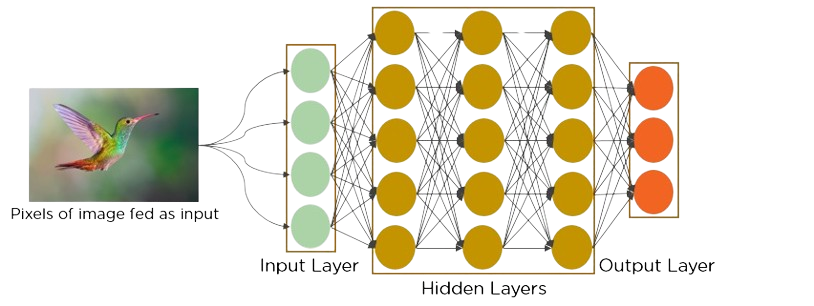
\includegraphics[width=\columnwidth]{cnn}
	\caption{A example of bird classification pipeline.}
	\label{fig:cnn}
\end{figure}

\section{Dataset}
\label{sec:dataset}
In order to conduct research, I decided to begin with a specific region's avian population. The dataset used for this research is sourced from Kaggle and is publicly available under the name ``\textbf{Indian-Birds-Species-Image-Classification}''[\ref{fig:birds}]. This dataset encompasses a wide variety of bird species that are native to India, totaling 25 distinct species. Some noteworthy species included in this dataset are the Asian Green Bee-eater, Indian Peacock, Common Kingfisher, and the Indian Grey Hornbill, among others.

This dataset is comprehensive, containing a total of 37,000 images that have been carefully categorized and divided into training and validation sets. Specifically, 30,000 images are allocated for training purposes, while the remaining 7,500 images are reserved for validation, adhering to an 8:2 split ratio. Each bird species is well-represented in the dataset, with a total of 1,500 images per species. This robust dataset serves as a fundamental resource for conducting image classification tasks and facilitates the development and refinement of machine learning models aimed at accurately identifying and classifying various bird species indigenous to India.
%------------------------------------------------------------------------
\section{Methodology}
\label{sec:method}
This project is multifaceted, incorporating various network structures, optimizers, schedulers, data augmentation methods, and training strategies to cultivate a robust and effective model.

\subsection{Architectures}
\label{method:arch}
Different network architectures showcase distinct characteristics and performance attributes. These differences can significantly impact the network's capabilities and suitability for specific tasks and applications.

\subsubsection{VGG}
VGG[\ref{fig:vgg}], also known as VGGNet, proposed by Simonyan and Zisserman\cite{simonyan2014very} at Oxford's Visual Geometry Group, is a convolutional neural network model[\ref{fig:vggm}] that proves increasing network depth could enhance performance to some extent.  It distinctly illustrates that a deeper network can significantly bolster performance, especially evident in its VGG16 and VGG19 variants\cite{simonyan2014very}[\ref{fig:vggm}]. A hallmark of VGG is its unique employment of multiple stacked 3x3 convolution kernels as opposed to the larger 7x7 or 5x5 kernels[\ref{fig:vggk}]. This strategic design choice enhances parameter efficiency and bolsters the model's ability to capture complex patterns. Consequently, VGG has established itself as a robust model for visual recognition tasks. Despite these advancements, VGG’s profound network depth results in substantial computational demands and considerable memory usage, largely due to the extensive fully connected layers.
\begin{figure}[h]
	\centering
	\subfloat[]{\label{fig:vggm}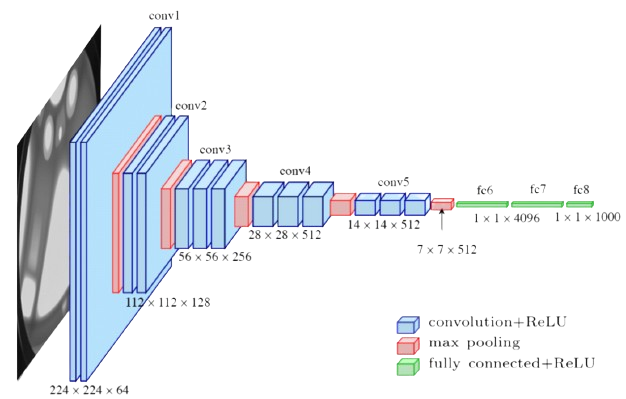
\includegraphics[width=0.7\columnwidth]{vgg}}
	\subfloat[]{\label{fig:vggk}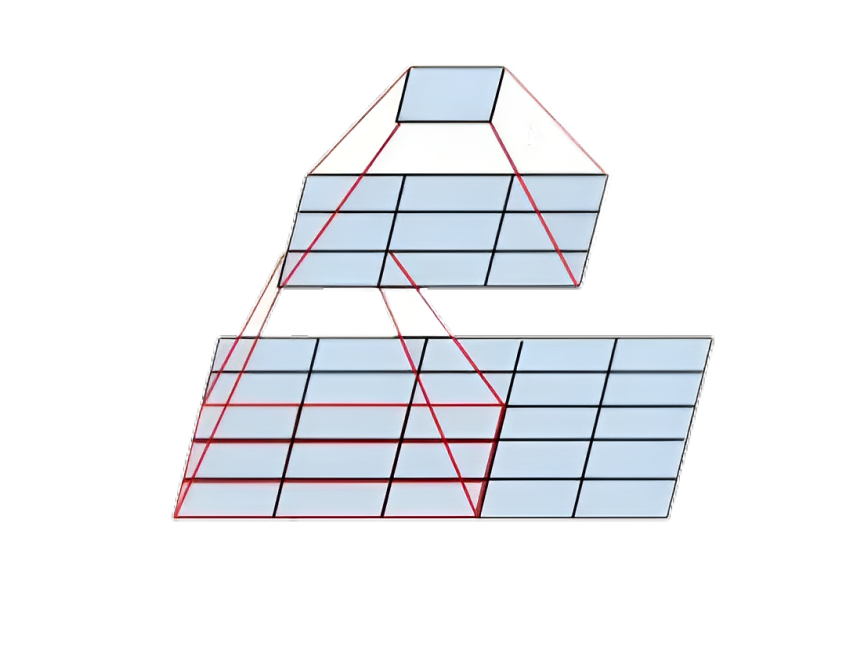
\includegraphics[width=0.3\columnwidth]{vgg_kernel}}
	\caption{Left is the architecture of VGGNet, right demonstrates 2 3x3 kernels replace 1 5x5 kernel\cite{simonyan2014very}.}
	\label{fig:vgg}
\end{figure}

\subsubsection{ResNet}
ResNet[\ref{fig:resblock}], also known as Residual Network, introduced by He \etal\cite{he2016deep} at Microsoft Research, revolutionized neural network architecture, addressing the vanishing gradient problem\cite{he2016deep, simonyan2014very} in deep networks. Its design is accentuated by ``shortcut'' or ``skip connections''[\ref{fig:resblock}], allowing information to bypass layers, enhancing gradient flow and facilitating residual learning\cite{he2016deep}. This innovation simplifies the network optimization process and improves performance. Variants like ResNet-18, 34, 50, 101, \etc, demonstrate its adaptability, featuring various depths and structures. The architecture incorporates residual blocks or ``bottlenecks'' and ``shortcut'' connections that promote the efficient learning of identity functions, enabling the construction of networks with hundreds of layers without complicating optimization.
\begin{figure}[h]
	\centering
	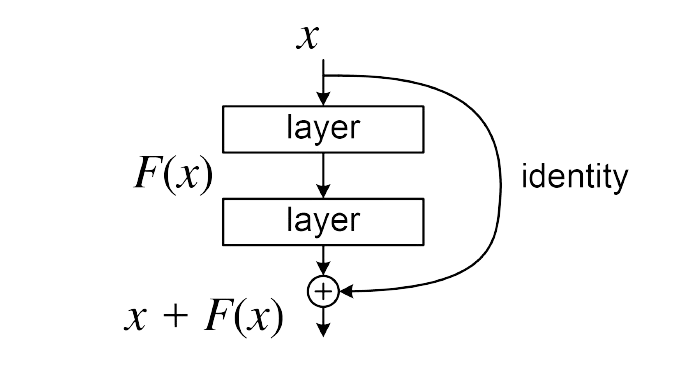
\includegraphics[height=0.3\columnwidth]{resblock}
	\caption{A typical ResBlock\cite{he2016deep}.}
	\label{fig:resblock}
\end{figure}

\subsubsection{EfficientNet}
EfficientNet[\ref{fig:eff}], proposed by Tan and Le\cite{tan2019efficientnet} at Google Research, innovatively employing a compound coefficient for coordinated scaling of network width, depth, and resolution, cultivating a nexus of enhanced performance and computational prudence. Built upon a foundation fortified by AutoML Neural Architecture Search (NAS) and pivotal components like Inverted Bottleneck MBConv, it executes meticulous grid searches, deriving coefficients that facilitate a harmonized scaling aligned with computational resources\cite{tan2019efficientnet}[\ref{fig:eff}]. EfficientNet unfurls a spectrum of nuanced models, with each manifestation, from B0 to B7, seamlessly balancing computational demands and performance. Armed with distinctive elements such as the Swish activation function\cite{tan2019efficientnet, ramachandran2017searching}, EfficientNet delineates a new paradigm in CNN architectures, establishing unprecedented standards in model scalability, accuracy, and computational efficacy.

\begin{figure}[h!]
	\centering
	\subfloat[]{\label{fig:eff-base}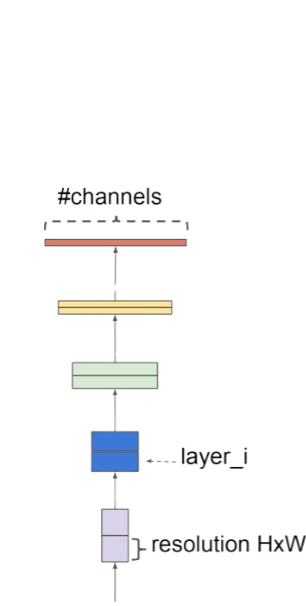
\includegraphics[width=0.2\columnwidth,height=0.2\columnwidth]{efficientnet-base}}
	\subfloat[]{\label{fig:eff-ws}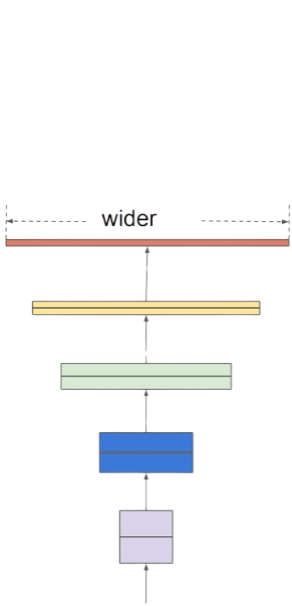
\includegraphics[width=0.2\columnwidth,height=0.2\columnwidth]{efficientnet-ws}}
	\subfloat[]{\label{fig:eff-ds}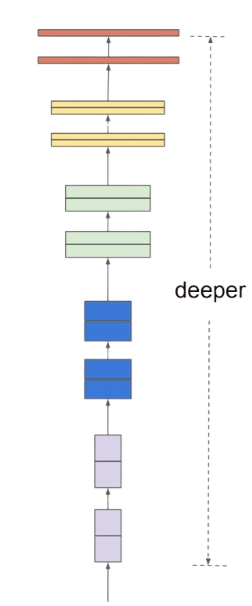
\includegraphics[width=0.2\columnwidth,height=0.2\columnwidth]{efficientnet-ds}}
	\subfloat[]{\label{fig:eff-rs}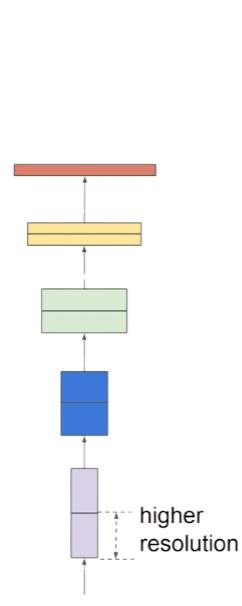
\includegraphics[width=0.2\columnwidth,height=0.2\columnwidth]{efficientnet-rs}}
	\subfloat[]{\label{fig:eff-cs}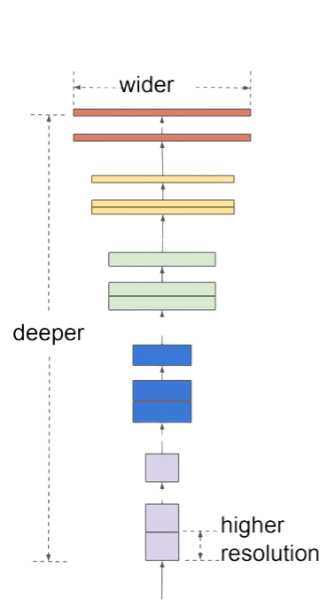
\includegraphics[width=0.2\columnwidth,height=0.2\columnwidth]{efficientnet-cs}}
	\caption{Different scaling methods in EfficientNet\cite{tan2019efficientnet}.}
	\label{fig:eff}
\end{figure}

\subsubsection{Vision Transformer}
Vision Transformer (ViT)[\ref{fig:vit}], introduced by Dosovitskiy \etal\cite{dosovitskiy2020image} at Google Research, is a notable development in computer vision, deriving from Transformer\cite{vaswani2017attention} architectures initially created for Natural Language Processing (NLP). It employs a Transformer-like architecture on image patches, especially for image classification. In this model, an image is segmented into fixed-size patches, which are linearly embedded and augmented with position embeddings, then processed through a standard Transformer encoder\cite{dosovitskiy2020image, vaswani2017attention}[\ref{fig:vit}, \ref{fig:swinvit}]. A typical Vision Transformer architecture further processes these patches along with a special token through a series of Transformer encoder blocks, with the token's representation being used to derive the output label post-processing. Unlike traditional convolutional and recurrent mechanisms, ViT utilizes the Transformer's attention mechanism, showcasing a novel approach in handling attention in computer vision, with the potential to work directly on images or in hybrid architectures alongside CNNs.
\begin{figure}[h]
	\centering
	\subfloat[]{\label{fig:vitm}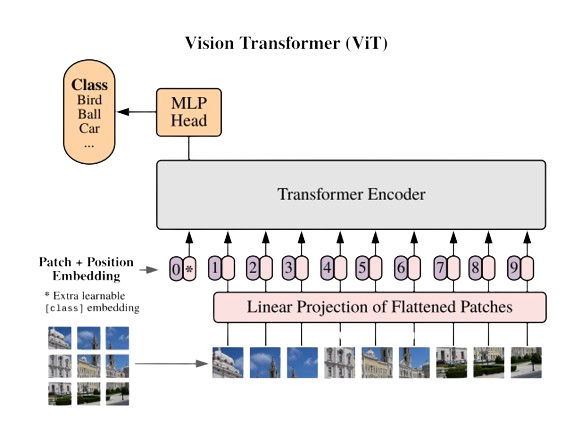
\includegraphics[width=0.7\columnwidth]{vit}}
	\subfloat[]{\label{fig:trans}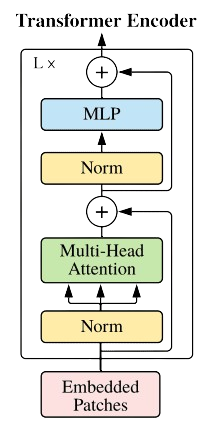
\includegraphics[width=0.3\columnwidth,height=0.5\columnwidth]{transformer}}
	\caption{Left is the architecture of ViT\cite{dosovitskiy2020image}, right is a Transformer block\cite{vaswani2017attention}}
	\label{fig:vit}
\end{figure}

\subsubsection{Swin Transformer}
Swin Transformer[\ref{fig:swin}], proposed by Liu \etal\cite{liu2021swin} at Microsoft Research Asia in 2021, adopts a hierarchical architecture with shifted windows for various scales and contexts in computer vision tasks. Initially, it employs Window Partitioning and Window-based Self-attention by segmenting images into non-overlapping windows and applying self-attention within each window\cite{liu2021swin, dosovitskiy2020image}[\ref{fig:swinvit}]. It then transitions to Shifted Window-based Self-attention\cite{vaswani2017attention}[\ref{fig:trans}], allowing window overlaps and enabling tokens to attend to neighboring windows. As it progresses through multiple stages, each comprising a certain number of Transformer layers, it hierarchically merges smaller windows into larger ones, reducing resolution while broadening the receptive field. Each stage corresponds to a feature map of a distinct resolution, making it a structured and flexible backbone for diverse vision tasks.
\begin{figure}[h]
	\centering
	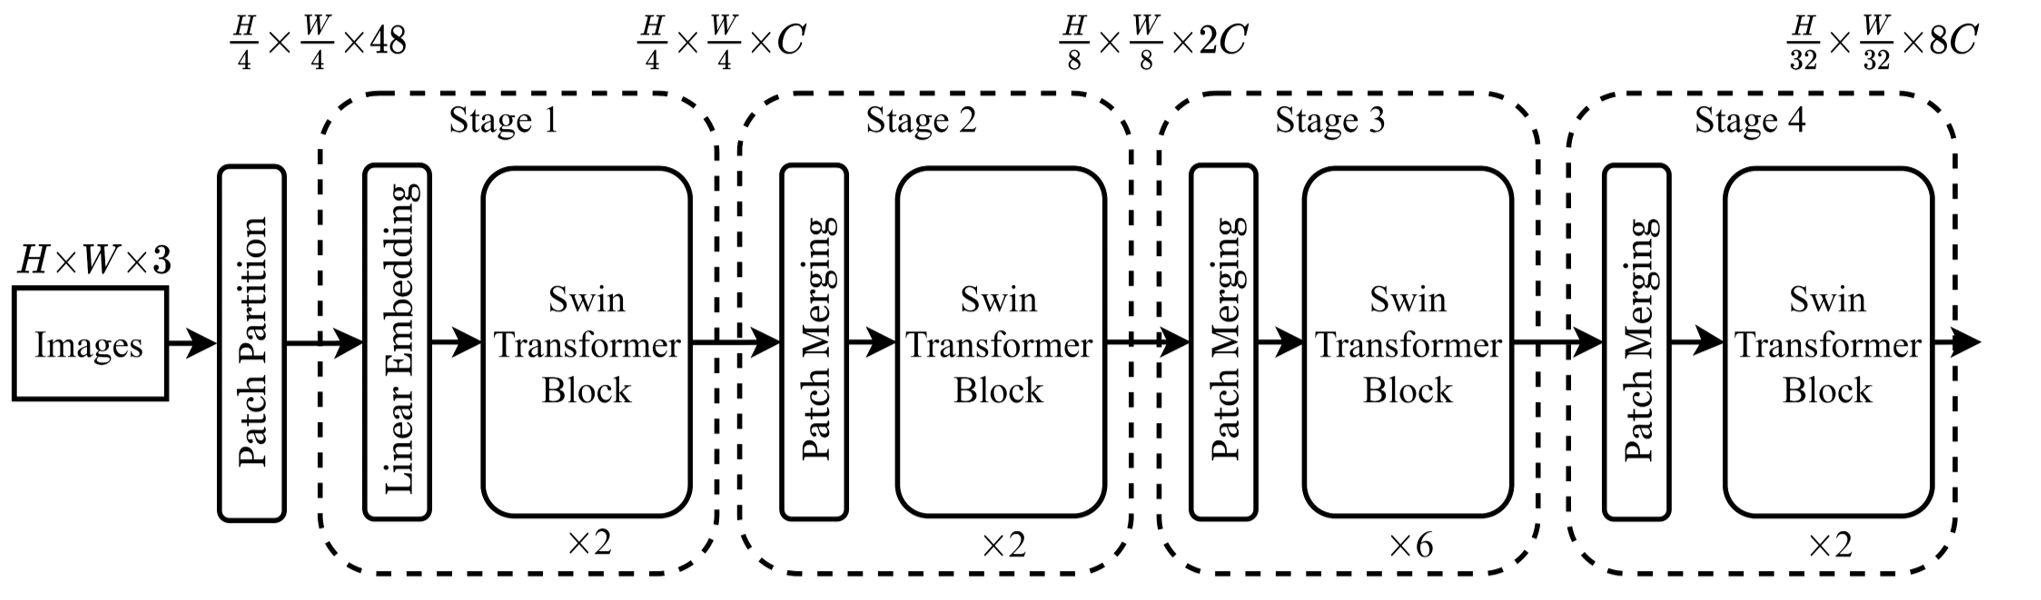
\includegraphics[width=\columnwidth]{swin}
	\caption{The architecture of Swin Transformer\cite{liu2021swin}.}
	\label{fig:swinm}
\end{figure}

Swin Transformer V2\cite{liu2022swin, liu2021swin}[\ref{fig:swinv2}] escalates capacity and resolution, integrating techniques like post-normalization, scaled cosine attention, and a log-spaced continuous position bias technique for stability in large vision models and effective model transfer across varying resolutions, marking a significant stride in enhancing the architecture and techniques for computer vision transformers.

\begin{figure}[h]
	\centering
	\subfloat[]{\label{fig:swinvit}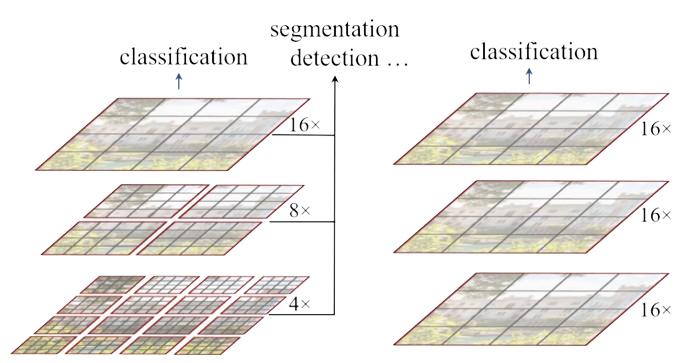
\includegraphics[width=0.5\columnwidth,height=0.5\columnwidth]{swin_vit}}
	\subfloat[]{\label{fig:swinv2}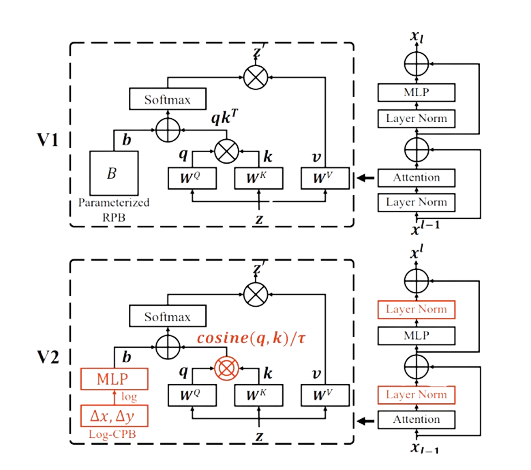
\includegraphics[width=0.5\columnwidth,height=0.5\columnwidth]{swinv2}}
	\caption{Left is the difference of patching methods between Swin and ViT\cite{liu2021swin, dosovitskiy2020image}, right is difference of customized Transformer blocks between Swin v1 and v2\cite{liu2022swin, liu2021swin}.}
	\label{fig:swin}
\end{figure}

\subsection{Strategies and Techniques}
\label{method:tech}
\subsubsection{Contrastive Learning and Triplet Loss}
Contrastive Learning and Triplet Loss are techniques used in machine learning to learn useful representations from data, often employed in self-supervised learning and similarity learning tasks.\\

\noindent\textbf{Contrastive Learning:}\\
\indent Contrastive Learning\cite{khosla2020supervised, hermans2017defense, dong2018triplet}[\ref{fig:triplet}] is a deep learning technique that focuses on learning representations by distinguishing similar instances from dissimilar ones in a representation space. It aims to bring representations of similar instances close together while pushing dissimilar instances far apart.\\

\noindent\textbf{Triplet Loss:}\\
\indent Triplet Loss\cite{hermans2017defense, dong2018triplet} is a distance-based loss function that operates on three data points: an anchor, a positive sample (similar to the anchor), and a negative sample (dissimilar to the anchor). The goal is to minimize the distance between the anchor and the positive sample while maximizing the distance between the anchor and the negative sample\cite{hermans2017defense, dong2018triplet}, thus learning embeddings that are closer for similar data and farther for dissimilar data.
Triplet Loss function shows following:
\[\ell(\mathbf{a},\mathbf{p},\mathbf{n}) = \mathbf{L} = \{l_1, \ldots, l_N\}^\top,\]
\[l_i = \max \{d(\mathbf{a}_i, \mathbf{p}_i) - d(\mathbf{a}_i, \mathbf{n}_i) + \text{margin}, 0\}\]
\[
\ell(\mathbf{x},\mathbf{y}) = 
\begin{cases} 
\text{mean}(\mathbf{L}), & \text{if reduction = `mean';} \\
\text{sum}(\mathbf{L}), & \text{if reduction = `sum'}.
\end{cases}
\]
where \( \mathbf{a}, \mathbf{p}, \) and \( \mathbf{n} \) (representing anchor, positive, and negative examples, respectively), and a nonnegative, real-valued function (“distance function”), \( N \) is the batch size; \( d \) is a nonnegative, real-valued function quantifying the closeness of two tensors, referred to as the distance\_function; and \( \text{margin} \) is a nonnegative margin representing the minimum difference between the positive and negative distances that is required for the loss to be 0.\\

\noindent\textbf{Pairwise Distance Function:}\\
\[
\text{pair dist}(\mathbf{x}, \mathbf{y}) = \left\| \mathbf{x} - \mathbf{y} + \varepsilon \right\|_p,
\]
where \( p \)-norm, with constant \( \varepsilon \) added to avoid division by zero if \( p \) is negative. When \( p \) is equal to \( 2 \), it is euclidean metric.\\

\noindent\textbf{Cosine Similarity Function:}\\
\[
\text{cos similarity} = \frac{\mathbf{x}_1 \cdot \mathbf{x}_2}{\max\left(\left\| \mathbf{x}_1 \right\|_2 \cdot \left\| \mathbf{x}_2 \right\|_2, \varepsilon\right)}.
\]
where \( \mathbf{x}_1 \) and \( \mathbf{x}_2 \) are two inputs, computed along dim.\\

\begin{figure}[h]
	\centering
	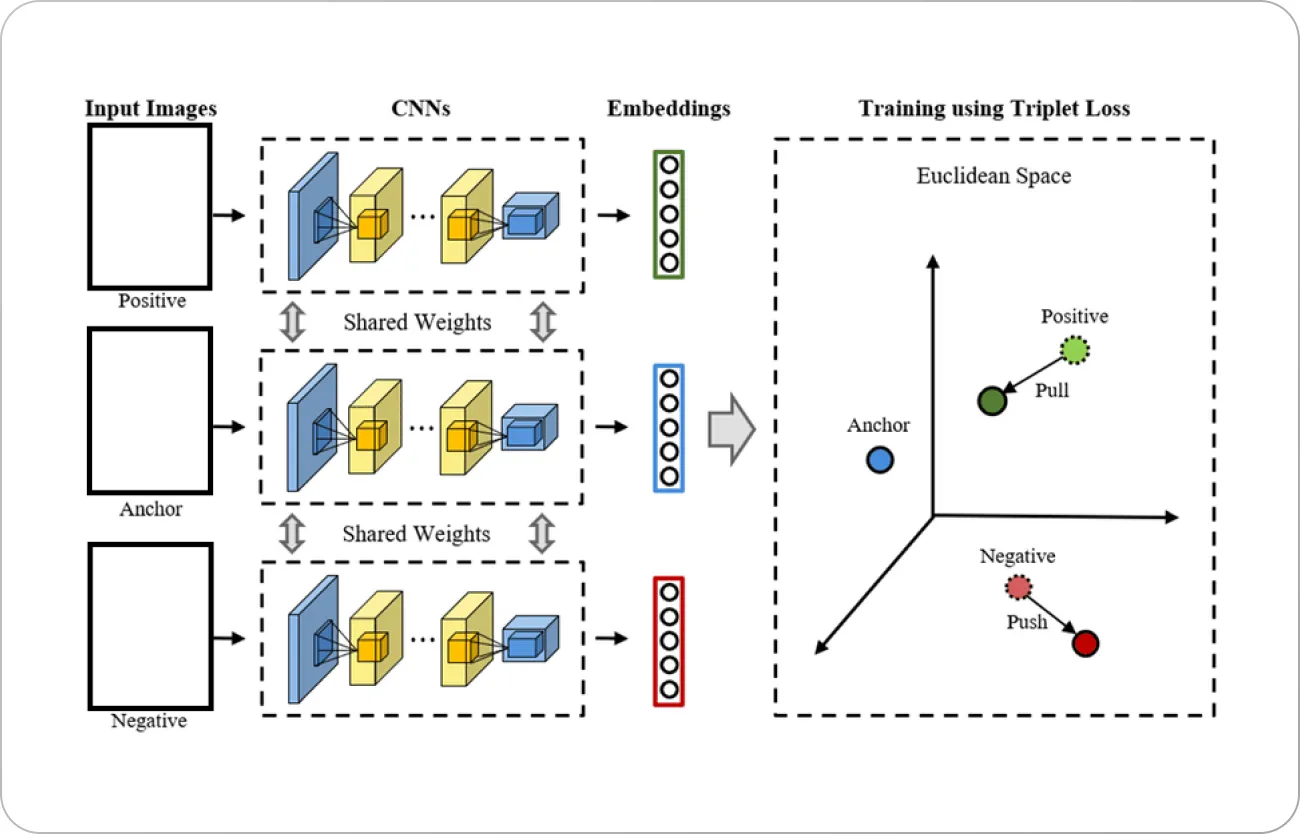
\includegraphics[width=\columnwidth,height=0.5\columnwidth]{triplet}
	\caption{A example of triplet trainning pipeline\cite{hermans2017defense}.}
	\label{fig:triplet}
\end{figure}

\subsubsection{Transfer Learning}
Transfer Learning\cite{weiss2016survey, zhuang2020comprehensive} is a key technique in deep learning, optimizing model performance without the extensive computational resources usually needed to train models from scratch. Widely used in computer vision and natural language processing, it leverages the foundational structures of pre-trained models, fine-tuning them for specific tasks\cite{weiss2016survey, zhuang2020comprehensive, simonyan2014very, he2016deep, tan2019efficientnet, dosovitskiy2020image, liu2021swin, liu2022swin}. This approach boosts computational efficiency and speeds up model training, achieving better performance by utilizing knowledge from pre-existing models. It's particularly valuable in scenarios with scarce or highly domain-specific data, and finds extensive use in varied applications like image and text classification, showcasing its importance and adaptability across numerous deep learning domains.

\subsubsection{Data Augmentation}
Data Augmentation is a technique employed to increase the variety and size of a training dataset by applying a range of transformations to the existing data, without the need for collecting new data. This strategy is pivotal for improving model generalization, reducing overfitting, and enhancing performance, particularly in scenarios with limited data.

In this project, the Albumentations library\cite{buslaev2020albumentations}[\ref{fig:album}] is leveraged to augment data using a variety of transformations from the Transforms module. The chosen transformations include Blur, Crop, Dropout, and Geometric transforms[\ref{fig:album}], which significantly enhance the diversity of the training dataset. Additionally, three different levels are set to simulate various situations. Through these transformations, the model encounters a broader spectrum of data variations, boosting its robustness and ability to handle real-world variances in input data, thereby aiding in better generalization on unseen data.

\begin{figure}[h]
	\centering
	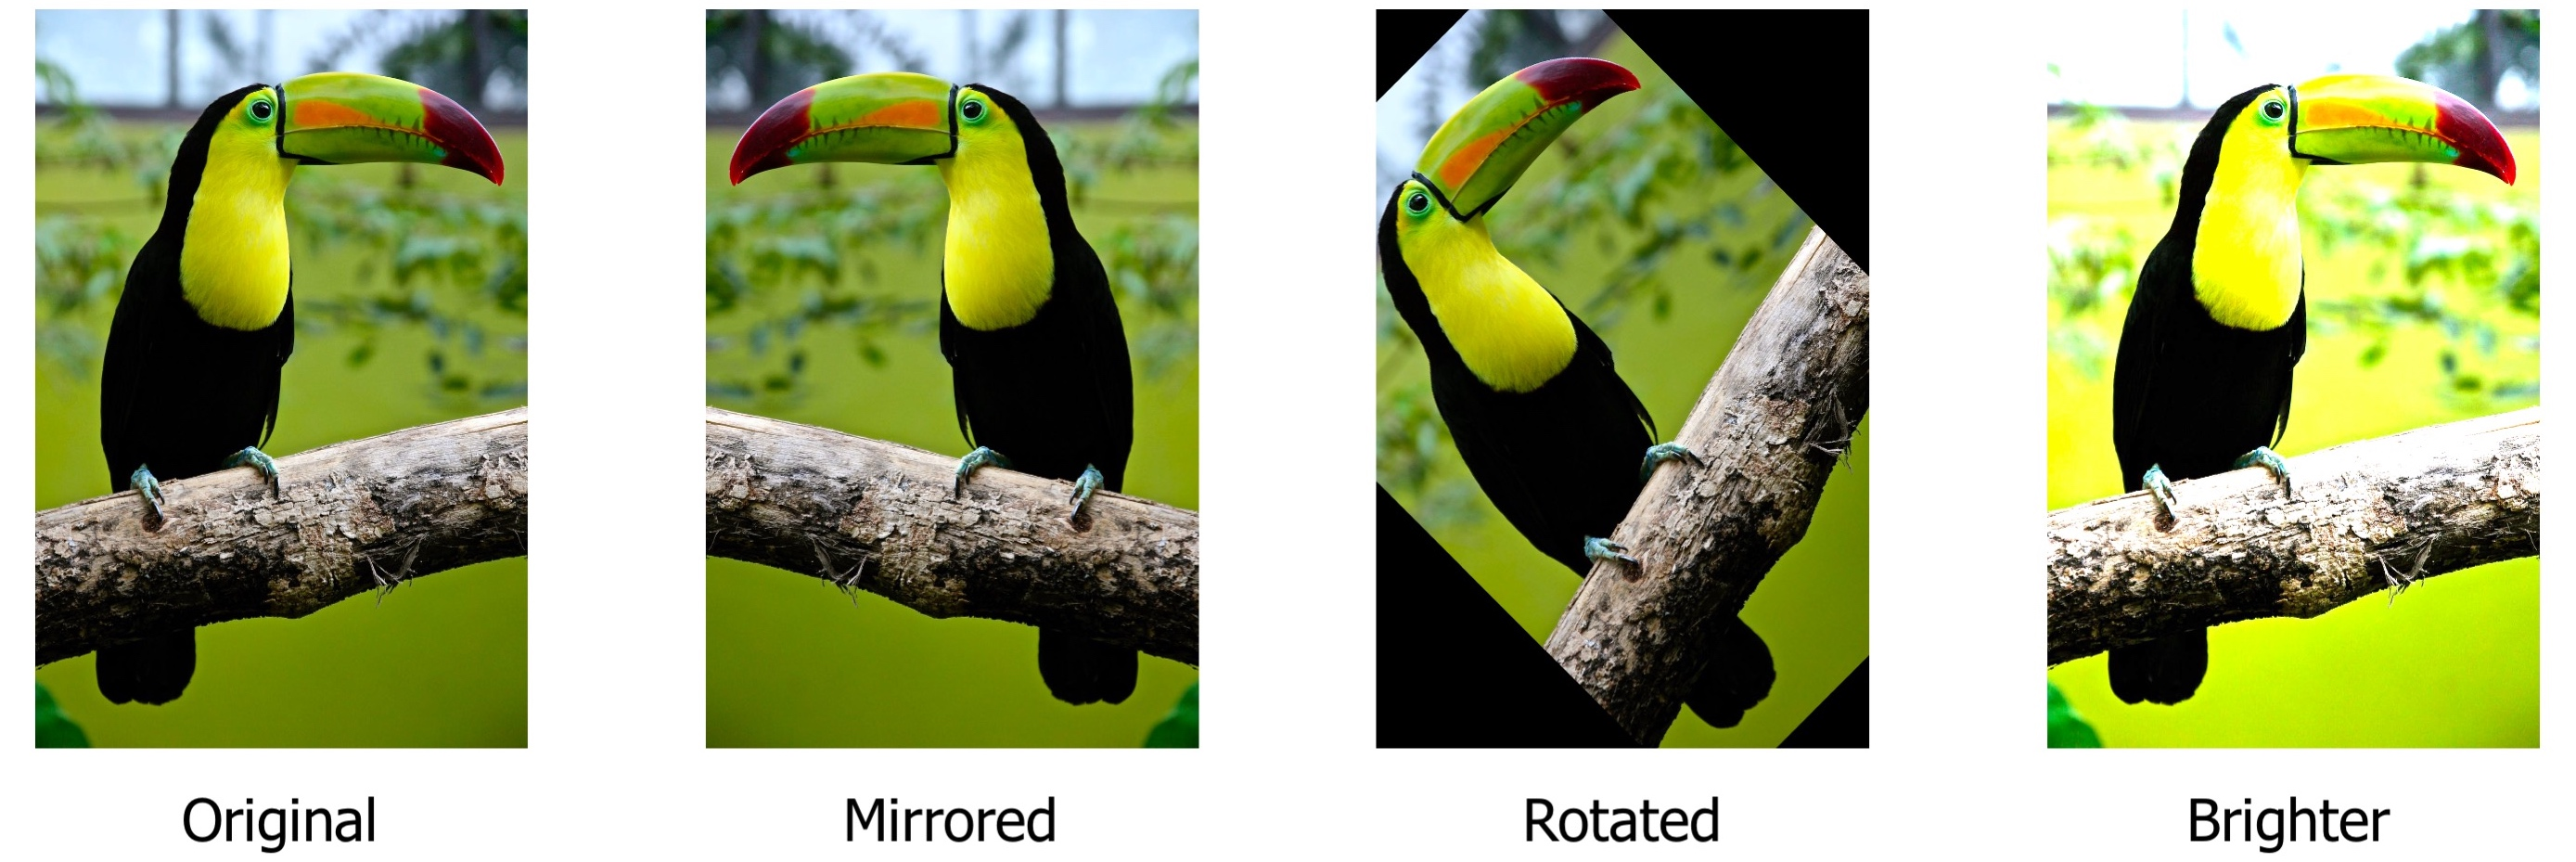
\includegraphics[width=\columnwidth]{album}
	\caption{Example of different type augmentations.}
	\label{fig:album}
\end{figure}

\subsubsection{Optimizer and LR Scheduler}
AdamW\cite{loshchilov2017decoupled, loshchilov2018fixing}[\ref{fig:adamw}] was chosen over Stochastic Gradient Descent (SGD)\cite{ruder2016overview} and Adam\cite{kingma2014adam} for its efficient handling of weight decay and computational efficiency. Unlike traditional L2 regularization, which requires manual addition of a regularization term to the loss, AdamW integrates this directly into the back-propagation formula, streamlining the optimization process. Compared to SGD, AdamW offers an adaptive learning rate mechanism, reducing the necessity for meticulous hyperparameter tuning. Unlike Adam, which falls short in its implementation of weight decay, AdamW addresses this shortcoming effectively, making it a more attractive choice for optimizing the model, especially in scenarios where computational resources are a concern\cite{loshchilov2017decoupled, loshchilov2018fixing}.

CosineAnnealingWarmRestarts\cite{loshchilov2016sgdr}[\ref{fig:cosann}] scheduler modulates the learning rate between an upper and lower bound (\(\eta_{\text{max}}\) and \(\eta_{\text{min}}\) respectively) using the formula\cite{loshchilov2016sgdr}:
\[ \eta_t = \eta_{\text{min}} + \frac{1}{2}(\eta_{\text{max}} - \eta_{\text{min}})(1 + \cos(\frac{T_{\text{cur}}}{T_i} \pi)) \]
where \( T_{\text{cur}} \) is the number of epochs since the last restart and \( T_i \) is the number of epochs between two warm restarts. This strategy allows for a dynamic learning rate that could help escape local minima and find better optima in the model's parameter space[\ref{fig:cosann}]. The warm restarts reset the learning rate to its initial value, promoting exploration of different parts of the parameter space and potentially aiding in avoiding local minima, which can be beneficial in scenarios with complex optimization landscapes.

\begin{figure}[h]
	\centering
	\subfloat[]{\label{fig:adamw}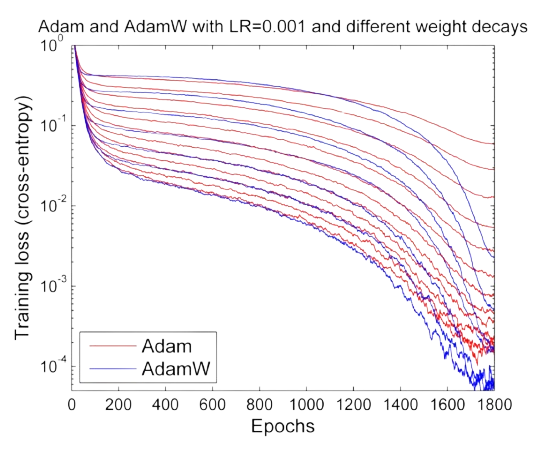
\includegraphics[width=0.5\columnwidth,height=0.5\columnwidth]{adamw}}
	\subfloat[]{\label{fig:cosann}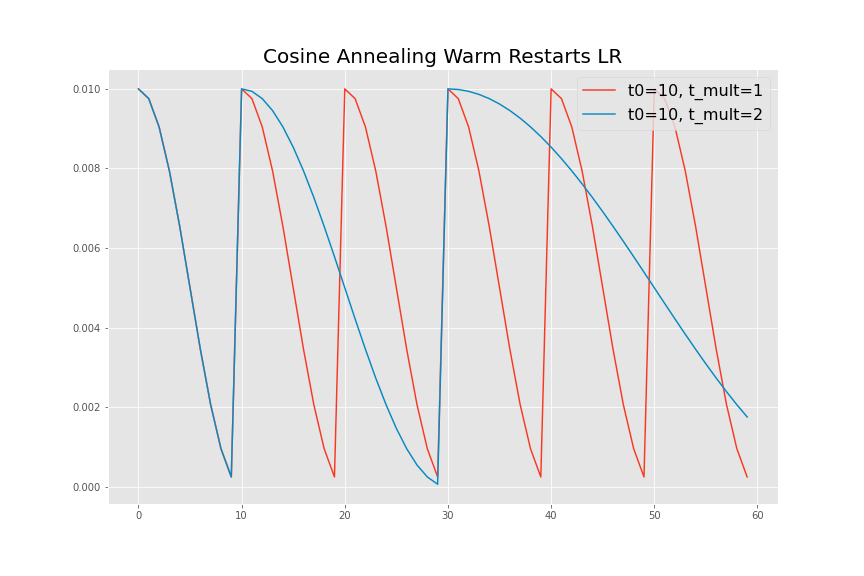
\includegraphics[width=0.5\columnwidth,height=0.5\columnwidth]{cosannwr}}
	\caption{Left compares AdamW with Adam\cite{loshchilov2017decoupled, loshchilov2018fixing, kingma2014adam}, right is a CosineAnnealingWR with $t_0=10$, $t\_mul=1,2$.}
	\label{fig:opt}
\end{figure}

\subsubsection{Stochastic Weight Averaging}
Stochastic Weight Averaging (SWA)\cite{izmailov2018averaging, huang2017snapshot}[\ref{fig:swa-clr}] is a technique derived from the idea of averaging model weights in the weight space to achieve superior models characteristics, unlike Fast Geometric Ensembling (FGE)\cite{izmailov2018averaging} which averages model outputs in the model space. Despite SGD\cite{ruder2016overview} potentially achieving lower training loss, SWA often results in lower test error rates, indicating better generalization. The key benefits of SWA include\cite{izmailov2018averaging, ruder2016overview}:
\begin{itemize}
    \item \textbf{Closer Proximity to Optimal Weight Space}: Moving closer to optimal weight space compared to standard SGD.
    \item \textbf{Efficient Prediction Phase}: Only requiring one computation during the prediction phase, akin to SGD.
    \item \textbf{Lower Test Error Rates}: Achieving lower test error rates, indicating better generalization compared to SGD.
    \item \textbf{Smooth Training Loss Landscape}: Contributing to a smoother training loss landscape, avoiding sharp increases in loss.
    \item \textbf{Performance Improvement with Minimal Training}: Achieving 0.6\%-0.8\% improvement on advanced models like ResNet-50, DenseNet-161, and ResNet150 with just 10 epochs of training on the ImageNet dataset.
\end{itemize}
These benefits, alongside SWA's ease of integration and cost-efficiency, make it a compelling choice for optimizing models in various projects.


\begin{figure}[h]
	\centering
	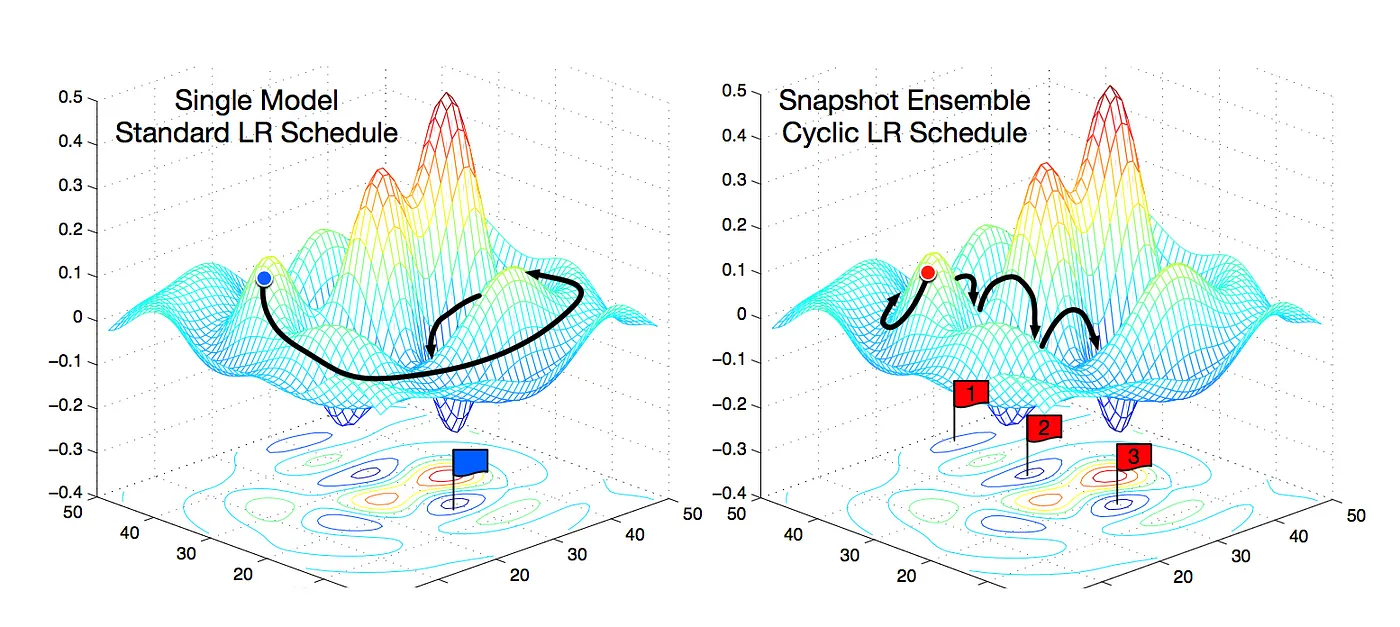
\includegraphics[width=\columnwidth]{swa-clr}
	\caption{Snapshot Ensembles\cite{huang2017snapshot, izmailov2018averaging, smith2017cyclical}.}
	\label{fig:swa-clr}
\end{figure}

\subsubsection{Learning Rate Finder}
Cyclical Learning Rates (CLR)\cite{smith2017cyclical, huang2017snapshot}[\ref{fig:swa-clr}] streamline the learning rate adjustment during training, reducing the need for manual fine-tuning. By cyclically varying the learning rate between specified bounds, CLR helps in faster convergence, aiding the model to escape saddle points and local minima, common challenges in training. This method leads to optimal accuracy with fewer iterations, enhancing training efficiency. The use of a triangular learning rate policy within CLR further simplifies the learning rate variation, making it an effective and practical approach for training models, especially in classification tasks. Through an LR range test, CLR also facilitates the identification of optimal learning rates, providing a computational advantage and improved model performance over traditional learning rate schedules\cite{smith2017cyclical}.

\subsubsection{Automatic Mixed Precision and BFLOAT16}
Automatic Mixed Precision (AMP)\cite{micikevicius2018mixed}[\ref{fig:amp}] accelerates neural network training and inference by employing lower precision arithmetic for most computations, and higher precision for critical operations, ensuring numerical stability and accuracy. This technique reduces memory usage and speeds up training, making it a practical solution for optimizing deep learning workflows.

BFLOAT16\cite{kalamkar2019study}[\ref{fig:bf16}] is a half-precision floating-point format that balances computational efficiency with a wide numerical range, similar to single-precision floating-point (FP32). It requires no hyper-parameter tuning for model convergence, unlike other lower precision formats, making it a favorable numeric format for accelerating deep learning training across various workloads, with easy integration into existing FP32-based projects.

Using Automatic Mixed Precision (AMP) and BFLOAT16\cite{micikevicius2018mixed, kalamkar2019study}[\ref{fig:amp-bf}] can speed up training and inference without losing accuracy, which is key for rapid model iterations or time-sensitive deployments. BFLOAT16, blending lower precision efficiency with higher precision numerical range, is ideal for handling diverse deep learning workloads.

\begin{figure}[h]
	\centering
	\subfloat[]{\label{fig:amp}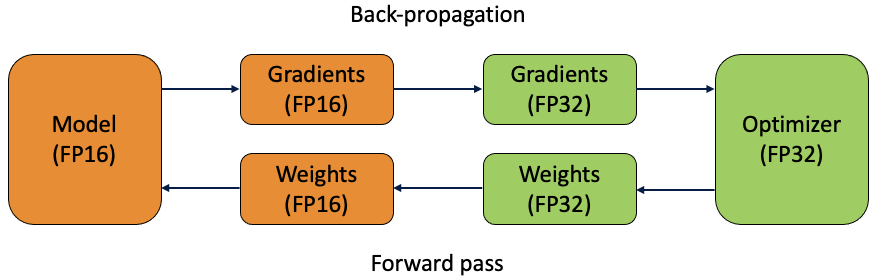
\includegraphics[width=0.5\columnwidth]{amp}}
	\subfloat[]{\label{fig:bf16}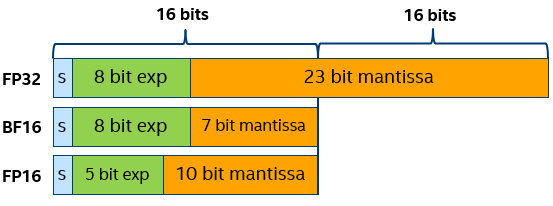
\includegraphics[width=0.5\columnwidth]{bf16}}
	\caption{Left is mixed-precision training pipeline\cite{micikevicius2018mixed}, right is a comparison between BF16 and others\cite{kalamkar2019study}.}
	\label{fig:amp-bf}
\end{figure}

%------------------------------------------------------------------------
\section{Experiments}
Through comprehensively testing various combinations and configurations, and by carefully observing and analyzing the experimental results, individuals can delve deeper into understanding the strengths, weaknesses, and nuances of different techniques. This iterative process of exploration and reflection not only helps in evaluating the effectiveness and applicability of these techniques in different contexts but also fosters a deeper comprehension of the underlying principles and mechanics
\label{sec:exper}
\subsection{Experiments Environment}
\label{exper:env}
The experimental platform consists of an AMD 7950X with 16 cores, 64GB RAM, and an NVIDIA RTX4090 with 24GB VRAM. The versions of PyTorch and Lightning used are 2.1.0, with a CUDA version of 12.1. All models were trained using BF16 mixed precision, and employed an early stopping strategy with a patience of 10.
Features like SWA, CLR, \etc are controlled through OmegaConf with yaml.
\subsection{Metrics}
\label{exper:metr}
Accuracy refers to the percentage of correct predictions out of the total samples. While accuracy can assess the overall correctness, it may not be a good indicator when dealing with imbalanced datasets.
\[Accuracy = \frac{TP+TN}{TP+TN+FP+FN}\]
\indent Precision represents the probability that a sample predicted as positive is actually positive. Precision measures the accuracy of positive predictions, while accuracy considers both positive and negative predictions.
\[Precision = \frac{TP}{TP+FP}\]
\indent Recall refers to the probability that an actual positive sample is predicted as positive. Higher recall indicates a higher probability of correctly identifying actual positive cases.
\[Recall = \frac{TP}{TP+FN}\]
\indent Specificity measures the proportion of actual negatives that are correctly identified. It quantifies the ability of the model to correctly identify negative instances, which is crucial in scenarios where false positives are to be minimized.
\[Specificity = \frac{TN}{TN+FP}\]
\indent The F1 score is designed to balance precision and recall, finding a trade-off point between the two.
\[F1-Score = \frac{2\times Precision\times Recall}{Precision+Recall}\]

\subsection{Results}
\label{exper:res}
\begin{tabularx}{\columnwidth}{lccccc}
	\toprule
	 & acc & prec & recall & spec & f1 \\
	\midrule
	effnet\_b0 & 0.8890 & 0.8893 & 0.8887 & 0.9954 & 0.8890 \\
	effnet\_b2 & 0.9376 & 0.9378 & 0.9374 & 0.9974 & 0.9376 \\
	effnet\_b4 & 0.9676 & 0.9677 & 0.9675 & 0.9986 & 0.9676 \\
	resnet34 & 0.8707 & 0.8709 & 0.8705 & 0.9946 & 0.8707 \\
	resnet50 & 0.9115 & 0.9116 & 0.9114 & 0.9963 & 0.9115 \\
	swinv2\_s & \textbf{0.9905} & \textbf{0.9906} & \textbf{0.9904} & \textbf{0.9996} & \textbf{0.9905} \\
	swinv2\_t & 0.9868 & 0.9869 & 0.9867 & 0.9994 & 0.9868 \\
	vgg16 & 0.9424 & 0.9425 & 0.9423 & 0.9976 & 0.9424 \\
	vgg19 & 0.9349 & 0.9350 & 0.9348 & 0.9973 & 0.9349 \\
	vit\_s & 0.9661 & 0.9662 & 0.9660 & 0.9986 & 0.9661 \\
	vit\_t& 0.8643 & 0.8644 & 0.8642 & 0.9943 & 0.8643 \\
	\bottomrule
	\end{tabularx}	
The table above shows the results without data augmentation. It is the outcome of training only the model's head while utilizing a pretrained encoder.

\begin{tabularx}{\columnwidth}{lccccc}
	\toprule
	 & acc & prec & recall & spec & f1 \\
	\midrule
	effnet\_b0 & 0.9905 & 0.9907 & 0.9903 & 0.9996 & 0.9905 \\
	effnet\_b2 & 0.9944 & 0.9945 & 0.9943 & 0.9997 & 0.9944 \\
	effnet\_b4 & 0.9947 & 0.9958 & 0.9949 & 0.9997 & 0.9958 \\
	resnet34 & 0.9727 & 0.9728 & 0.9726 & 0.9989 & 0.9727 \\
	resnet50 & 0.9853 & 0.9854 & 0.9852 & 0.9994 & 0.9853 \\
	swinv2\_s & \textbf{0.9959} & \textbf{0.9960} & \textbf{0.9958} & \textbf{0.9998} & \textbf{0.9959} \\
	swinv2\_t & 0.9934 & 0.9935 & 0.9933 & 0.9997 & 0.9934 \\
	vgg16 & 0.9763 & 0.9764 & 0.9762 & 0.9990 & 0.9763 \\
	vgg19 & 0.9810 & 0.9811 & 0.9809 & 0.9992 & 0.9810 \\
	vit\_s & 0.9922 & 0.9923 & 0.9921 & 0.9997 & 0.9922 \\
	vit\_t & 0.9852 & 0.9853 & 0.9851 & 0.9994 & 0.9852 \\
	\bottomrule
\end{tabularx}
The table above shows the results obtained when training the entire model using a pretrained encoder without any data augmentation.
~\\
~\\
\begin{tabularx}{\columnwidth}{lccccc}
	\toprule
	 & acc & prec & recall & spec & f1 \\
	\midrule
	b0\_aug\_fr & 0.9033 & 0.8993 & 0.9021 & 0.9014 & 0.8975 \\
	b0\_aug & \textbf{0.9845} & \textbf{0.9776} & \textbf{0.9764} & \textbf{0.9981} & \textbf{0.9787} \\
	\bottomrule
	\end{tabularx}	
The table above shows the results for the ``hard'' mode of data augmentation, using a pretrained encoder with the option to either enable or disable the freezing encoder setting.
~\\
~\\
\begin{tabularx}{\columnwidth}{lccccc}
	\toprule
	 & acc & prec & recall & spec & f1 \\
	\midrule
	b0\_drop & 0.9220 & 0.9221 & 0.9220 & 0.9968 & 0.9220 \\
	b0\_fr\_drop & \textbf{0.9785} & \textbf{0.9786} & \textbf{0.9785} & \textbf{0.9991} & \textbf{0.9785} \\
	b0 & 0.9035 & 0.9036 & 0.9035 & 0.9960 & 0.9035 \\
	b0\_fr & 0.9071 & 0.9072 & 0.9071 & 0.9961 & 0.9071 \\
	\bottomrule
	\end{tabularx}	
The table above illustrates the results of the ``easy'' mode data augmentation. It uses a pretrained encoder with three linear layers head. Two different techniques were applied: freezing the encoder and adding dropout and droppath layers.
~\\
~\\
\begin{tabularx}{\columnwidth}{lccccc}
	\toprule
	 & acc & prec & recall & spec & f1 \\
	\midrule
	b0\_all & \textbf{0.9335} & \textbf{0.9186} & \textbf{0.9112} & \textbf{0.9996} & \textbf{0.9307} \\
	\bottomrule
	\end{tabularx}	
	The table above represents the ``easy'' mode of data augmentation. In this mode, I used a pretrained encoder, used the last three linear layers as the model's head, applied dropout and drop path techniques, employed skip connections to connect features at different scales, and utilized triplet loss for training.
\section{Discussions and Conclusion}
\label{sec:discons}
Through comprehensive experiments, I have discovered that Transformer-based models and the EfficientNet series perform exceptionally well. This is because they have been trained extensively on large datasets or fine-tuned through an exhaustive search process, resulting in excellent feature extraction capabilities for images. Although the VGG series is relatively older and slower, it still performs well, partly due to its relatively high parameter count.

When using ResNet as a standalone feature extractor, its performance is moderate and is comparable to the smaller efficientNet\_b0 network in terms of parameter count. Additionally, increasing the number of classifier layers without freezing the encoder is not always effective. Conversely, applying dropout and droppath after freezing the encoder can yield good results.

Furthermore, I found that triplet loss is an effective technique. By monitoring the validation triplet loss, it becomes evident that the feature space distances are well-separated for different classes of input images after passing through the encoder, while images of the same class are closer together.

In addition, techniques like CosineAnnealing, SWA, and CLR have proven to be valuable in saving a significant amount of time during the training process.

%%%%%%%%% REFERENCES
	{\small
		\bibliographystyle{ieee_fullname}
		\bibliography{egbib}
	}

\end{document}
